\setcounter{topnumber}{5}
\setcounter{bottomnumber}{5}
\setcounter{totalnumber}{5}

\chapter{Procedimentos e resultados}

\centerline{\begin{minipage}[c]{\textwidth}
		\centering
		\noindent
		\captionof{figure}{Polarizçaõ da base}
		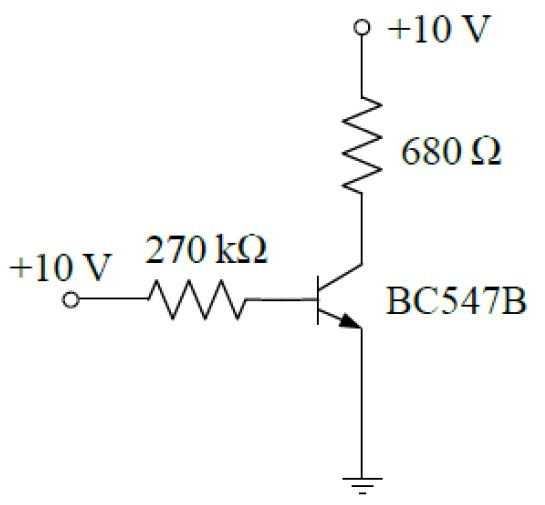
\includegraphics[width=0.5\textwidth]{Imagens/Figura1.jpg}
		\legend{Fonte: Produzido pelos autores}
		\label{Figura1}
\end{minipage}}

\centerline{\begin{minipage}[c]{\textwidth}
		\centering
		\noindent
		\captionof{figure}{Polarização por divisor de tensão}
		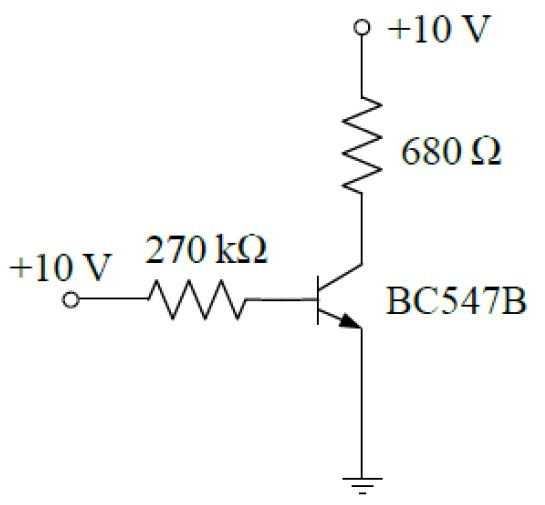
\includegraphics[width=0.5\textwidth]{Imagens/Figura1.jpg}
		\legend{Fonte: Produzido pelos autores}
		\label{Figura2}
\end{minipage}}


\begin{enumerate}
	\item Monte o circuito da Figura \ref{Figura1} e complete a terceira coluna da tabela \ref{Tabela1}.

	
	\centerline{\begin{minipage}[c]{\textwidth}
			\centering
			\noindent
			\captionof{table}{Valores teóricos e práticos do circuito da Figura \ref{Figura1}}
			\begin{tabular}{cccccc}
				\toprule
				Variável & Valor teórico & Valor prático & Erro (\%) \\
				\midrule \midrule
				$V_C$ &  $ 3,02V $ & $ 5,32V $ & $1,5 \% $ \\
				\midrule
				$V_B$ &  $ 0,7V $ & $ 0,67V $ & $1,5 \% $ \\
				\midrule
				$V_E$ &  $ 0V $ & $ 0,015V $ & $1,5 \% $ \\
				\midrule
				$V_{CE}$ &  $ 3,02V $ & $ 5,32 V $ & $1,5 \% $ \\
				\midrule
				$I_{C}$ &  $ 10,26mA$ & $ 6,87 mA $ & $ 699 \% $ \\
				\midrule
				$I_{B}$ &  $ 34,44\mu A $ & $ 34,44\mu A $ & $ 1,55\% $ \\
				\midrule
				$\beta_{CC}$ & $ 298 $ & $ 298 $ & $ 87,68 \% $ \\
				\midrule
				$P_D$ &  $ 30,98 mW $ & $ 36,54mW $ & $ \% $ \\
				\midrule
				\bottomrule
			\end{tabular}%
			\legend{Fonte: Produzido pelos autores}
			\label{Tabela1}
	\end{minipage}}

	\item Aqueça o transistor e monitore o valor da corrente $ I_C $. Tal parâmetro varia significativamente?
	
	
	
	\item Monte o circuito da Figura \ref{Figura2} e complete a terceira coluna da Tabela \ref{Tabela2}.
	
	
		\centerline{\begin{minipage}[c]{\textwidth}
			\centering
			\noindent
			\captionof{table}{Valores teóricos e práticos do circuito da Figura \ref{Figura2}}
			\begin{tabular}{cccccc}
				\toprule
				Variável & Valor teórico & Valor prático & Erro (\%) \\
				\midrule \midrule
				$V_C$ &  $ 7,25V $ & $ 7,18V $ & $1,5 \% $ \\
				\midrule
				$V_B$ &  $ 2,69V $ & $ 2,68V $ & $1,5 \% $ \\
				\midrule
				$V_E$ &  $ 1,992V $ & $ 2,015V $ & $1,5 \% $ \\
				\midrule
				$V_{CE}$ &  $ 5,26V $ & $ 5,16V V $ & $1,5 \% $ \\
				\midrule
				$I_{C}$ &  $ 1,98mA$ & $ 2,01 mA $ & $ 699 \% $ \\
				\midrule
				$I_{B}$ &  $ 6,66\mu A $ & $9,61\mu A $ & $ 1,55\% $ \\
				\midrule
				$\beta_{CC}$ & $ 298 $ & $ 298 $ & $ 87,68 \% $ \\
				\midrule
				$P_D$ &  $ 10,41mW $ & $ 10,37mW $ & $ W\% $ \\
				\midrule
				\bottomrule
			\end{tabular}%
			\legend{Fonte: Produzido pelos autores}
			\label{Tabela2}
	\end{minipage}}

	\item Aqueça o transistor e monitore o valor da corrente $ I_C $. Tal parâmetro varia significativamente?
	
	\item Calcule os erros das suas medidas e complete as Tabelas \ref{Tabela1} e \ref{Tabela2}. Considere que o erro é dado por
		
		$$\%\; de\; erro = \frac{valor \; prático - valor \; teórico}{valor \; teórico} \times 100$$
	\item  Qual circuito apresenta erros menores? Tal fato coincide com o que foi visto nas aulas teóricas?
	
	\item Qual circuito é mais estável do ponto de vista térmico? Por que isso ocorre?
	
	\item O transistor bipolar utilizado nesta experiência apresenta diferentes valores de ganho de corrente quando opera nos circuitos das Figuras \ref{Figura1} e \ref{Figura2}. Por que tal fato ocorre?
	
	\item Quais sãos as possíveis fontes de erro desta experiência?
	
\end{enumerate}